\section{Introduction}
\label{introduction}


% state the learning objective
\par The aim of this laboratory assignment is to analyse a RC circuit, which contains a sinusoidal voltage source $v_s$ and a capacitor $C$. The other components present in this four mesh circuit are 7 resistors (from $R_1$ to $R_7$) and a linearly dependent current $I_b$ and voltage $V_d$ sources.
\par The voltage controlled current source depends on the constant $K_d$ and the current controlled voltage source has a linear dependence on the constant $K_b$.

\par The voltage source varies in time as it follows:

\begin{equation}
v_s(t) = V_s u(-t) + sin(2 \pi f t)u(t)
\label {equation:n1}
\end{equation}
where
\begin{equation}
u(t)=e
\begin{cases}
0 & $t$ < $0$ \\
1 & $t $\geq$ 0$
\end{cases}
\label {eq:n2}
\end{equation}

\par The data generated automatically by the Python script is given in the table below.

\begin{table}[ht]
  \centering
  \begin{tabular}{|l|r|}
    \hline    
    {\bf Name} & {\bf Value} \\ \hline
    R1 & 1.041113e+03 \\ \hline
R2 & 2.099452e+03 \\ \hline
R3 & 3.131091e+03 \\ \hline
R4 & 4.119470e+03 \\ \hline
R5 & 3.115588e+03 \\ \hline
R6 & 2.047994e+03 \\ \hline
R7 & 1.027544e+03 \\ \hline
Vs & 5.068716e+00 \\ \hline
C & 1.041275e-06 \\ \hline
Kb & 7.287471e-03 \\ \hline
Kd & 8.115684e+03 \\ \hline

  \end{tabular}
  \caption{Initial data generated by Python script. All variables are expressed in Ohms, V, F, S or A.}
  \label{tab:initial_data}
\end{table}



\par The nodes (from $V_1$ to $V_8$) are displayed as it shows in Figure \ref{tab:initial_data}. The fourth node is considered to be the ground one.


\par
   

\par
The report is subdivided in three major sections.
\par The first, the theoretical analysis(\ref{section:theo}). This section adresses, sequencially, the nodal analysis, then the calculus of $R_eq$. With these results, the natural response of the circuit, the forced response are computed, and then superimposed. To finish, it is made a study of the frequency response of the circuit.
\par The second, the simulation analysis(\ref{section:sim}). In order to validate the results obtained in section \ref{section:theo}, operating point, transient and then frequency analysis are made.
\par The study of the circuit is concluded with a careful comparison between the results obtained using the different tools, in section \ref{section:comp}.
The conclusions of this study are outlined in the final section (\ref{section:con}).



\begin{figure}[ht] \centering
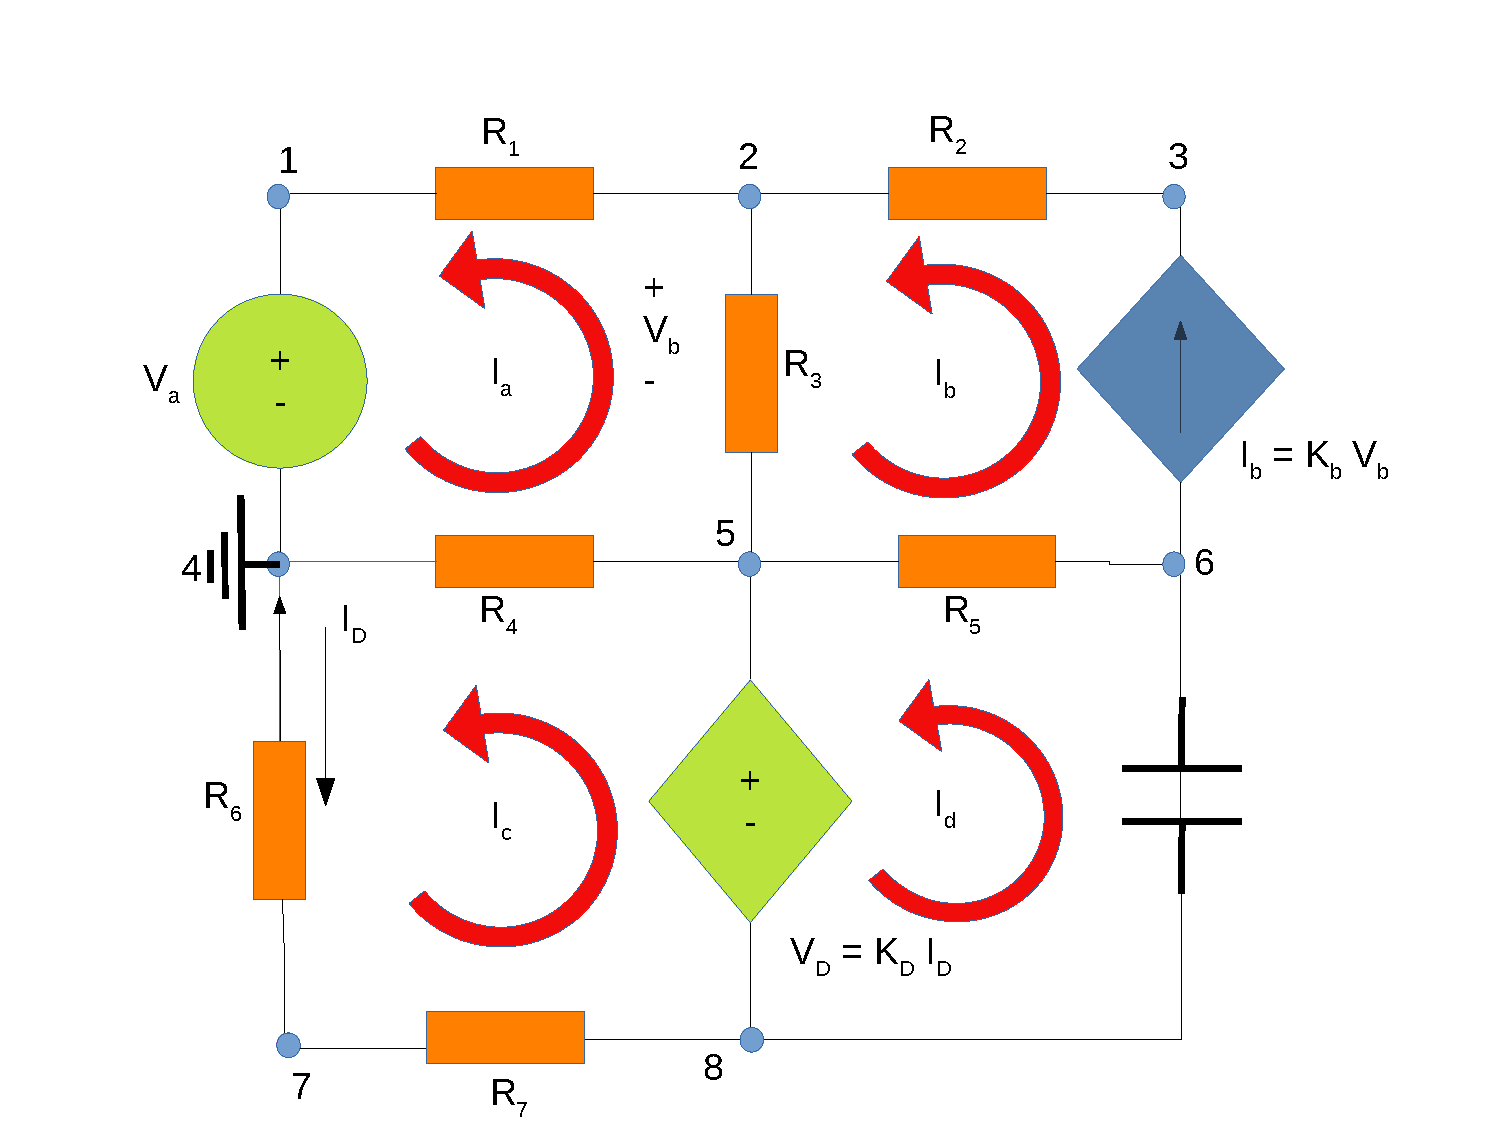
\includegraphics[width=0.8\linewidth]{t2draw.pdf}
\caption{ RC Circuit analysed.}
\label{RC Circuit.}
\end{figure}
\par 
   

\newpage
















